
\section{Espectrometría de fluorescencia}

\subsection{Instrumentación: el espectrofluorímetro}

Para caracterizar la respuesta óptica de una sustancia, generalmente se desea registrar tanto el espectro de excitación como el de emisión. 
El instrumento científico por excelencia para realizar estas mediciones es el espectrofluorímetro. 
Fundamentalmente, este instrumento permite realizar mediciones de la intensidad de luz que emite una muestra, haciendo escaneos en longitud de onda de emisión y excitación.
Adicionalmente, algunos pueden realizar mediciones de timepo de vida resueltas en el timpo, escaneos sincrónicos con alguna señal y mediciones de anisotropía en la polarización de materiales luminiscentes.
Estas capacidades son fundamentales para investigaciones en diversas disciplinas científicas, incluyendo química, bioquímica, farmacología, ciencias ambientales, ciencia de materiales y biomedicina.
El objetivo principal de un espectrofluorímetro es obtener los espectros de emisión y de excitación de una muestra.
Para lograr este objetivo, el instrumento debe ser capaz de iluminar la muestra con múltiples longitudes de onda diferentes y registrar su respuesta a cada una de ellas.

La Figura 2.1 muestra un diagrama esquemático de un espectrofluorímetro genérico.
Este instrumento incluye todos los componentes clave para cumplir su función. 
Utiliza una lámpara de espectro amplio que funciona como fuente de luz de alta intensidad para un rango extenso de longitudes de onda. 
Posteriormente la luz es filtrada por un monocromador de excitación que permite seleccionar la longitud de onda con la que se desea iluminar a la muestra.
La luz de excitación seleccionada se enfoca sobre la muestra colocada en la cámara principal, cuya luminiscencia, generalmente con una longitud de onda mayor que la luz de excitación, es filtrada por el monocromador de emisión.
Los monocromadores suelen estar motorizados, lo que permite que el escaneo sea automático. 
La luz restante llega a un detector, usualmente un tubo fotomultiplicador (PMT), un detector muy sensible que convierte fotones en corriente eléctrica.
El espectrofluorímetro emplea diversas técnicas para reducir la luz parásita (longitudes de onda diferentes a la deseada), como el diseño en ángulo de 90° entre los brazos de excitación y emisión, y un compartimento hermético pintado de negro no reflectante.
La señal del PMT es procesada electrónicamente, digitalizada y analizada en una computadora. 
Este sistema también controla los monocromadores y la adquisición de datos, además de permitir al usuario ajustar parámetros y facilitar la visualización y análisis de los datos.
A menudo, se incorporan componentes adicionales en el camino óptico, como obturadores, polarizadores, divisores de haz y otros elementos ópticos, para estudiar diferentes propiedades de la muestra.

\begin{enumerate}
    \item que mide un espectrofluorimetro?
    \item cuales son sus componentes?
    \item que variables puede controlar?
\end{enumerate}

\begin{SCfigure}
     \centering
     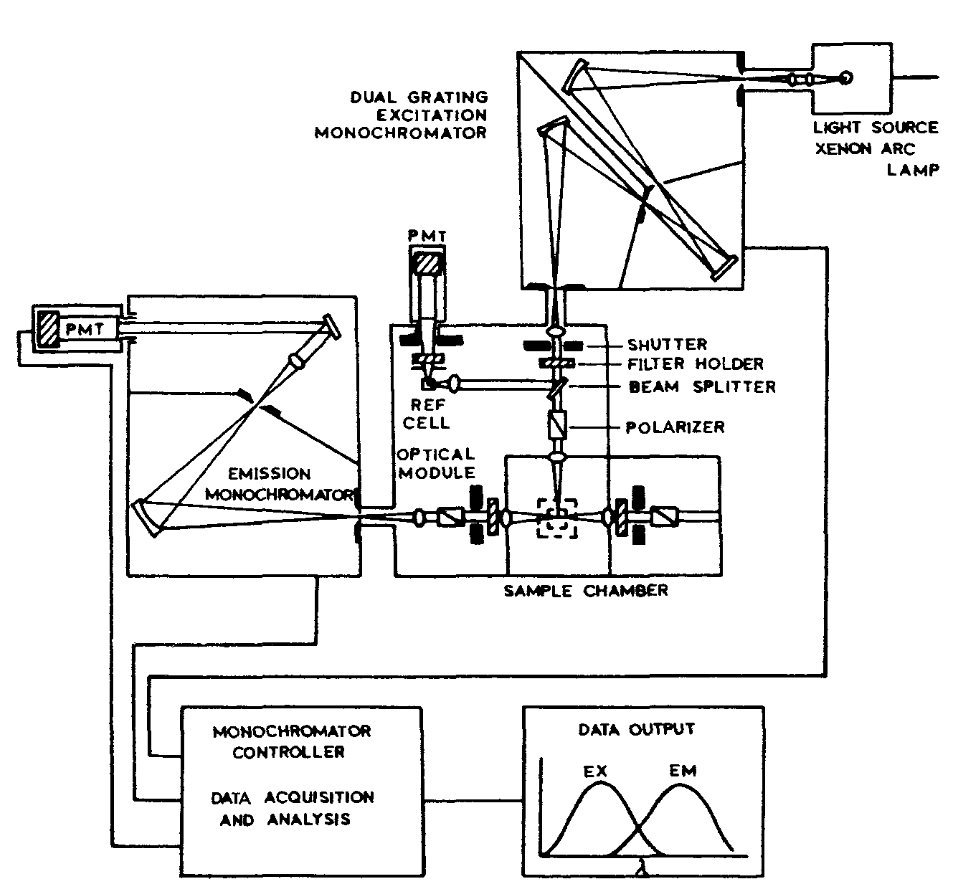
\includegraphics[width=0.6\textwidth]{spectrometer_diagram_lako.png}
     \caption{
    \textbf{Diagrama de un espectrofluorímetro genérico}
    \todo{Trabajar en estafigura}
    (\textbf{A}) Diagram of the Horiba PTI QuantaMaster hardware. Red arrows represent motors and limit switch connectors, black is BNC, blue is USB and orange represents a fiber optic. The path that light takes inside the spectrometer is represented in thick blue arrows. 
    (\textbf{B}) and (\textbf{C}) Representation of the old and new instrumental control module respectively.
    (\textbf{D}) Representation of the raw signal measured from the PMT detector.
    (\textbf{E}) Spectrum of the sample constructed from the raw signals measured at each wavelength.
    }
     \label{fig:spec_diagram_lako}
\end{SCfigure}


\subsection{Medición de tiempos de vida: \textit{Time-Correlated Single Photon Counting} (TCSPC) \todo{va a la intro}}

Muchos espectrofluorímetros comerciales tienen la capacidad de medir el tiempo de vida de los fluoróforos con tiempos típicos del orden de los nanosegundos. 
Sin embargo, debido a las transiciones prohibidas de los lantánidos (\todo{Ver cap N}) el tiempo de vida de las UCNPs es del orden de los cientos de microsegundos.
Aunque esto alivia la necesidad de una electrónica rápida y costosa, contradictoriamente hace que no se pueda medir su tiempo de vida en instrumentos comerciales, ya que los valores típicos están muy alejados del rango en el que operan \cite{bujjamer2020}.

Existen distintas técnicas para medir el tiempo de vida \cite{becker_fluorescence_2012}, pero la más implementada es \textit{Time-Correlated Single Photon Counting} (TCSPC).
Como la técnica se suele aplicar para tiempos de vida del orden de los nanosegundos es común que se usen componentes de electrónica rápida 
Usualmente la explicación de esta técnica involucra introducir múltiples componentes de electrónica rápida que son necesarios para medir tiempos del orden de nanosegundos.
Como en nuestro caso esos componentes no son necesarios, daremos una explicación simplificada.
TCSPC es una técnica digital que cuenta fotones correlacionados temporalmente con respecto a un pulso de excitación.
El experimento comienza con un pulso de excitación, que tiene dos tareas fundamentales: (i) excitar a la muestra y (ii) iniciar algún tipo de cronómetro.
La muestra se excita repetidamente utilizando una fuente de luz pulsada, a menudo un láser o una lámpara de destellos.
Cada pulso es monitoreado, produciendo una señal de inicio que activa el contador del cronómetro.
La rampa de voltaje se detiene cuando se detecta el primer fotón de fluorescencia proveniente de la muestra.
El TAC proporciona un pulso de salida cuyo voltaje es proporcional al tiempo transcurrido entre las señales de inicio y parada.
Un analizador multicanal (MCA) convierte este voltaje en un canal de tiempo utilizando un convertidor analógico a digital (ADC).
Sumando sobre muchos pulsos, el MCA genera un histograma de probabilidad de cuentas frente a los canales de tiempo.


\subsection{Epectrofluirimetros en argentina y obsolescencia}

Actualmente, el Departamento de Física de la FCEyN-UBA no cuenta con espectrofluorímetros para la caracterización de espectros de excitación y emisión.  
Para realizar este tipo de mediciones, la facultad dispone del laboratorio de fotoquímica del \todo{INQUIMAE}, que cuenta con tres espectrofluorímetros con distintas características, pero que tienen algo en común: ningún equipo tiene menos de 20 años, el más antigüo llegando a los 40 años de uso.
La disparidad en al antigüedad y funcionalidad de los instrumentos es un fenómeno común en laboratorios de investigación en países como Argentina, donde la inversión en ciencia es escasa o poco regular en el tiempo \cite{cioccaRealityScientificResearch2017}. 
Ante esta realidad, los institutos suelen priorizar la adquisición de equipos con nuevas capacidades, en lugar de renovar instrumentos existentes por versiones más modernas.  
Esto es posible gracias a la precisión y robustez de las partes mecánicas de los instrumentos, pero la obsolescencia de los equipos antiguos plantea problemas a largo plazo, especialmente cuando sus plataformas de control quedan desactualizadas.  
Con el tiempo, se vuelve complicado operar estos instrumentos, ya que los mecanismos de extracción de datos, como los disquetes, dejan de estar disponibles en el mercado. 
Aún más crítico es que el funcionamiento del equipo depende de la computadora de control, la cual utiliza placas y puertos que ya no se fabrican ni se consiguen en el mercado actual.  
El problema de la obsolescencia en instrumentos científicos afecta desproporcionadamente a instituciones con bajo presupuesto, ampliando la brecha de accesso a instrumentos de investigación avanzados.

Esto ha llevado a un auge en el desarrollo de instrumentos científicos accesibles y de bajo costo \cite{wenzel_open_2023, arancio_inequalities_2023}, particularmente en áreas como instrumentación, microscopía, espectroscopía y adquisición de datos \cite{jameson_fluorescent_1989, li_optical_2022, hu_fluorescent_2022}.
Las iniciativas de hardware abierto hacen que los diseños y la documentación estén disponibles de forma gratuita para que cualquier persona pueda usarlos, construirlos y modificarlos \cite{powell_democratizing_2012, oellermann_open_2022}.
Por ejemplo, la plataforma Arduino ha proporcionado una plataforma de desarrollo de electrónica económica y fácil de usar basada en un microcontrolador (https://www.arduino.cc/).
El OpenFlexure Microscope es un microscopio de código abierto que cuesta menos de 100 USD construir \cite{collins_robotic_2020}.
Asimismo, recientemente se desarrolló un espectrómetro basado en Raspberry Pi que cuesta menos de 400 EUR \cite{tunens_optical_2024}.
El software y los lenguajes de código abierto, como Python (http://www.python.org), que cuentan con bibliotecas numéricas y de instrumentación como NumPy \cite{harris_array_2020} y PyVISA \cite{grecco_pyvisa_2023}, han desempeñado un papel clave al reducir las barreras de entrada y facilitar la creación rápida de prototipos.
Cabe destacar que han surgido empresas enfocadas en hardware parcialmente o completamente abierto. Por ejemplo, OpenBCI (https://openbci.com/), que ofrece sistemas EEG de bajo costo para interfaces cerebro-computadora, y Opentrons (https://opentrons.com/), que proporciona soluciones de manejo de líquidos para la automatización de laboratorios.

En este capítulo de la tésis se explica detalladamente la plataforma de fuente abierta que desarrollamos para renovar la electrónica y el \textit{software} de control del espectrofluorímetro Horiba PTI QuantaMaster (QM) 400, uno de los espectrofluorímetros antigüos del laboratorio de fotoquímica del INQUIMAE.
Además de su renovación, ampliamos sus capacidades para medir tiempos de vida del orden de los microsegundos, que junto con el agregado de un láser pulsado externo de 980 nm nos permitió conseguir la plataforma ideal para la caracterización óptica de UCNPs tanto estática como dinámica.

\section{Renovación y ampliación de Horiba PTI Quanta Master 400 \todo{mencionar a juan}}

\subsection{Espectrofluorímetro Horiba PTI Quanta Master 400}

La serie Horiba PTI QM incluye espectrofluorímetros modulares para investigación científica y sistemas optimizados para mediciones de fotoluminiscencia.
Estos espectrofluorímetros se encuentran frecuentemente en los laboratorios de Argentina, por ejemplo, sabemos que hay tres equipos de esta serie en el laboratorio de fotoquímica del INQUIMAE (QM400, QM-4 y RatioMaster), dos en \todo{CIBION} y uno en \todo{CAC-CNEA}, y probablemente haya más de modelos similares en otras instituciones.
Al ser modelos antigüos y descontinuados se pueden encontrar en el mercado por precios que rondan los \$5000 USD, un costo relativamente bajo para un espectrofluorímetro científico.
Los bajos costos se dan por su antigüedad y fin de soporte por parte de la empresa, lo que obliga a los usuarios a resolver ellos mismos los problemas que haya con los equipos.
Por ejemplo, en CIBION, uno de los dos modelos que tienen no está funcionando porque hay problemas con la inicialización de los controladores en la PC.
En este trabajo, reacondicionamos específicamente un espectrofluorímetro QM 400 de más de 30 años de antigüedad,  (diagrama en la \textbf{Fig. \ref{fig:ref-diagram}A} y fotografía en la \textbf{Fig. \ref{fig:hardware}A}), pero dada la similaridad entre los distintos modelos de esta serie, la renovación se pueden aplicar a cualquiera de ellos con leves modificaciones. 

El QM 400 está equipado con una lámpara de xenón de 75 W como fuente de luz, la cual proporciona un amplio espectro de longitudes de onda (desde el infrarrojo cercano, alrededor de 1000 nm, hasta el ultravioleta, alrededor de 300 nm).
Los monocromadores de excitación y emisión contienen redes de difracción rotadas por motores paso a paso de 200 pasos por revolución, con especificaciones de 7 V y 0.7 A por bobina (M1 y M2), lo que permite una resolución en la selección de longitudes de onda de 0.5 nm. 
Ambos incluyen un fin de carrera electromecánico para verificar si se ha alcanzado la longitud de onda máxima.
Los motores paso a paso, junto con sus fines de carrera respectivos, están conectados a un módulo controlador de motores (MDM) mediante conectores propietarios no documentados. 
Los fotones son detectados por un tubo fotomultiplicador (PMT, modelo PTI 810), conectado al MDM a través de un cable BNC y polarizado con 1000 V desde una fuente de alimentación externa proporcionada también por el MDM. 
Esto genera pulsos negativos de alrededor de 170 ns con una terminación de 50 Ohm y un voltaje de −3.5 V (\textbf{Fig. \ref{fig:ref-diagram}D}). 
Finalmente, el MDM está conectado mediante un cable plano a una tarjeta de interfaz ISA en una PC con sistema operativo Windows 95 y el programa FelixGX, un \textit{software} propietario de adquisición y control instalado por Horiba (\textbf{Fig. \ref{fig:ref-diagram}B}).
FelixGX permite medir espectros de emisión y excitación (\textbf{Fig. \ref{fig:ref-diagram}E}), además de brindar herramientas de análisis rápido de los datos y controlar diferentes periféricos.

La antigüedad de la PC y electrónica de control hace que el proceso de adquisición de datos sea tedioso, y más aún para la caracterización de UCNPs.
Para hacer una medición el usuario debe colocar la muestra en la cámara y luego configurar en FelixGX un barrido de la longitud de onda de excitación o emisión.
En el caso de medir \textit{upconversion} se debe agregar un láser controlado externamente por una fuente de corriente (\textbf{Fig. \ref{fig:ref-diagram}A}) en la que se debe configurar por separado los parámetros de excitación, como la potencia.
Una plataforma de caracterización óptica completa de UCNPs debería ser capaz de medir espectros de excitación a 980 nm con distintas densidades de potencia, y tiempos de vida (también a distintas potencias) del orden de los microsegundos.
Además, como las mediciones de espectro y tiempo de vida son de larga duración (en especial a bajas potencias), resulta ideal que la plataforma permita configurar múltiples mediciones sucesivas sin la necesidad de una configuración manual por el usuario.
En las siguientes secciones, explicaremos los cambios de \textit{hardware} y \textit{software} que realizamos en el espectrofluorímetro para que sea una plataforma ideal para medir \textit{upconversion}.


%\todo{ \\
%serie horiba quantamaster. frecuencia de aparición en exactas y arg en general, baratos, etc. quizás mencionar lo de stefani \\
% \\
%componentes de funcionamiento: conectores originales, lampara, monocromadores, chamber, pmt, especificaciones \\
% \\
%software de control: felix gx, capacidades fundamentales y deficiencias \\
% \\
%que falta para caracterizar ucnps? time-consuming experiments, operación, medición de tiempos de vida, etc \\
%}

\begin{figure}[btp]
     \centering
     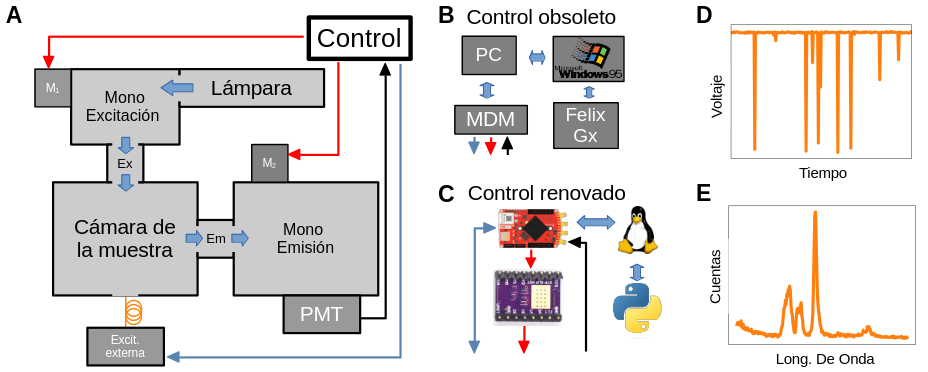
\includegraphics[width=\textwidth]{spec_diagram.png}
     \caption{
     \textbf{Representación esquemática del espectrofluorímetro}
     (\textbf{A}) Diagrama del hardware del Horiba PTI QM 400. Las flechas rojas representan los conectores de motores y fines de carrera, las negras corresponden a BNC, las azules a USB y las naranjas representan fibra óptica. La trayectoria de la luz dentro del espectrómetro está indicada con flechas azules gruesas.
     (\textbf{B}) y (\textbf{C}) Representación del módulo de control instrumental antiguo y nuevo, respectivamente.
     (\textbf{D}) Representación de la señal cruda medida por el detector PMT.
     (\textbf{E}) Espectro de la muestra construido a partir del conteo de picos en las señales crudas medidas para cada longitud de onda.
    }
     \label{fig:ref-diagram}
\end{figure}

\begin{figure}[h]
     \centering
     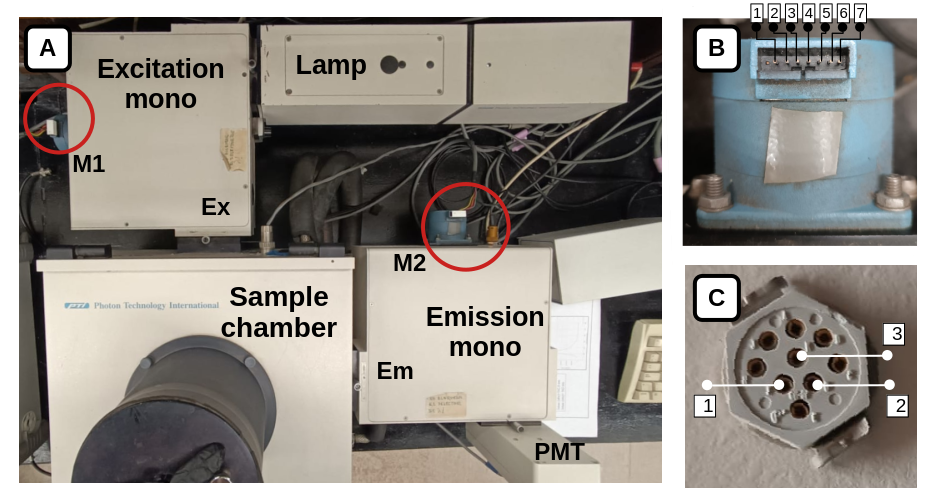
\includegraphics[width=0.9\textwidth]{hardware.png}
     \caption{\textbf{Horiba PTI QuantaMaster 400 picture}. \todo{maybe pasar a apéndice} (\textbf{A}) Picture of the whole spectrometer. Circled in red the monochromators' motors and limit switches. (\textbf{B}) Stepper motors pin diagram. The only used pins for the refurbished version are 1 and 7, and 3 and 5, which correspond to each motor winding respectively. (\textbf{C}) Limit switches pin diagram.}
     \label{fig:hardware}
\end{figure}


\subsection{Hardware para renovación}

Luego de hacer una inspección de todas las partes, decidimos conservar los componentes ópticos, la motorización, el PMT, la fuente de alta tensión y el chasis, ya que son robustos y funcionales.  
En contraste, la electrónica de control y detección resultó ser voluminosa, de código cerrado y obsoleta, por lo que optamos por reemplazarla con alternativas modernas: una microCPU con FPGA integrada Red Pitaya (RP) STEM LAB 125-14.
La RP cuenta con cuatro entradas y salidas analógicas que emiten y procesan señales en las radiofrecuencias, y un conjunto de pines digitales que permiten controlar circuitos integrados fácilmente (\textbf{\ref{fig:connection_diagram}}).
Esta placa junto con dos circuitos integrados DRV8825 que simplifican el control de los motores por paso cumplen la tarea de controlar a los monocromadores.
Este cambio en la electrónica de control nos permitió reemplazar el voluminoso módulo MDM ($\sim$10 cm $\times$ 30 cm $\times$ 30 cm) por dos controladores DRV8825 soldados a una placa PCB mucho más pequeña (10 cm$\times$ 10 cm $\times$ 2 cm)(\textbf{Fig. \ref{fig:placa}}).
Para facilitar la conexión de los componentes del espectrofluorímetro a la RP también agregamos a la placa un puerto IDC que permite conectar los pines digitales, y conectores a los motores a través de fichas adaptadas a medida.
El PMT se conecta a través de un cable BNC-SMA a uno de los canales analógicos de radiofrecuencias de la RP, luego son digitalizados por su conversor analógico digital (ADC)(\textbf{Fig. \ref{fig:ref-diagram}D}) y luego contados por software (\textbf{Fig. \ref{fig:ref-diagram}E}).
El ADC de 14 bits de la RP se configura con una frecuencia de muestreo de 32.25 MHz de forma tal de satisfacer el criterio de Nyquist.
La API de la RP permite configurar dos métodos distintos para comenzar una adquisición de datos.
Una opción es llamar a una función que comienza la adquisición de inmediato.
Alternativamente, se puede configurar una de las entradas analógicas o digitales como \textit{trigger} para comenzar una medición.
Nosotros usamos un método para medir espectros estáticos y otro para medir tiempos de vida.
Asimismo, la RP tiene dos mecanismos distintos para escribir los datos en la memoria al hacer una adquisición: un método por defecto de escritura a un espacio de memoria de 2$^{14}$ enteros de 16 bits, y un método de adquisición de memoria profunda (DMA) que permite guardar hasta 2 MB \cite{DMA_rp}.
Con esta capacidad para almacenar datos, a 32.25 MHz la ventana temporal de pulsos más grande que se puede obtener es de $\sim 0.5$ ms y $\sim 8$ ms respectivamente.
Aunque resulta beneficioso el método DMA y se podría implementar en esta renovación, nosotros utilizamos el método por defecto por la simplicidad que significó durante el desarrollo.
Para contrarrestar la corta duración de la ventana de adquisición, el software de control que desarrollamos permite agregar una demora para obtener ventanas de medición más grandes (ver sección \ref{sec:proceso_dinamico}).
El apéndice \ref{apendice:instrucciones_armado} explica detalladamente cómo reproducir las conexiones.

\begin{figure}
     \centering
     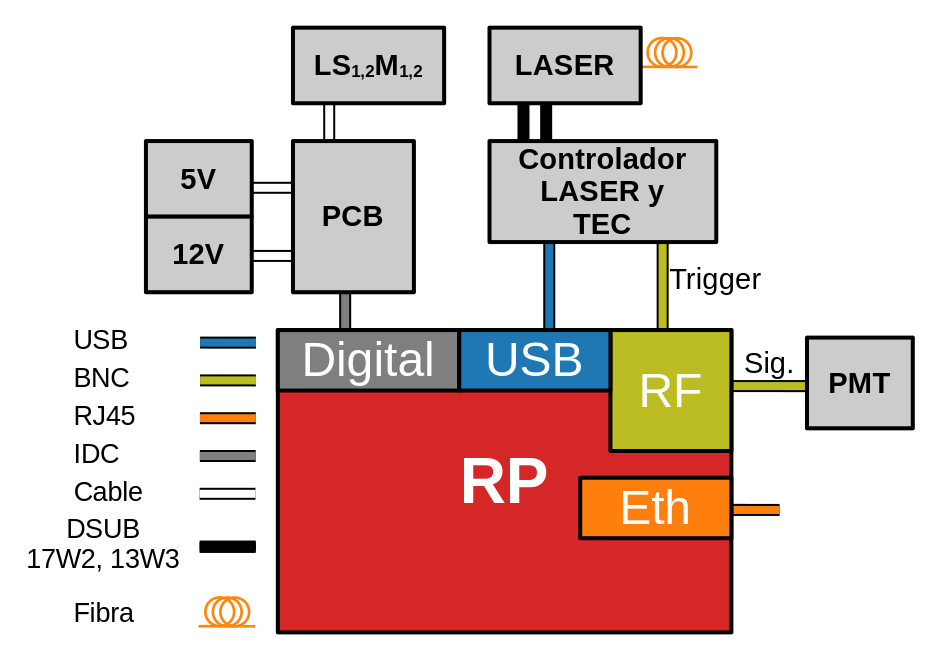
\includegraphics[width=0.8\textwidth]{connection_diagram.png}
     \caption{
    \textbf{Conexiones necesarias para la renovación y ampliación del QM400.}
    }
     \label{fig:connection_diagram}
\end{figure}


%\todo{Qué reemplazamos y con qué nos quedasmos, especificaciones finales}

\subsection{Hardware ampliación}

El espectrofluorímetro original QM 400 disponible en el laboratorio no era adecuado para estudiar \textit{upconversion}, ya que no contaba con una fuente de luz en el infrarrojo (IR). 
Tampoco era posible realizar mediciones de tiempos de vida de la luminiscencia debido a la falta de excitación pulsada y detección dependiente del tiempo. 
Luego de aplicar renovación mencionada anteriormente, incorporamos estas funcionalidades al equipo y al \textit{software} de forma independiente.

Para ello, añadimos una fuente de luz IR externa modulable al sistema. 
En nuestro caso, utilizamos un controlador de diodo láser y temperatura (TEC) de banco THORLABS ITC4020, controlado por la RP, para operar un diodo láser BL976-SAG300 de 976 nm y 300 mW. 
La salida del diodo láser se conecta mediante una fibra óptica a la entrada de fuente externa del QM 400 (\textbf{Fig. \ref{fig:ref-diagram}A}). 
El ITC4020 permite configurar la frecuencia de pulsado y el ciclo de trabajo, además de proporcionar una señal TTL que está en 5 V cuando el láser está prendido y 0 V cuando está apagado.
Esta señal se conecta a otra de las entradas analógicas de la RP, que luego la utiliza como \textit{trigger} para sincronizar la finalización de la excitación del láser, con la medición de los pulsos eléctricos de los fotones, para luego realizar histogramas y así medir los tiempos de vida, proceso que se explica en detalle en la sección \ref{sec:proceso_dinamico}.  

%\todo{ \\
%Excitación con laser pulsado. Control de potencia y duty cycle. funcionamiento del trigger. el resto ya lo puede hacer la RP \\
%}

\begin{figure}[h]
     \centering
     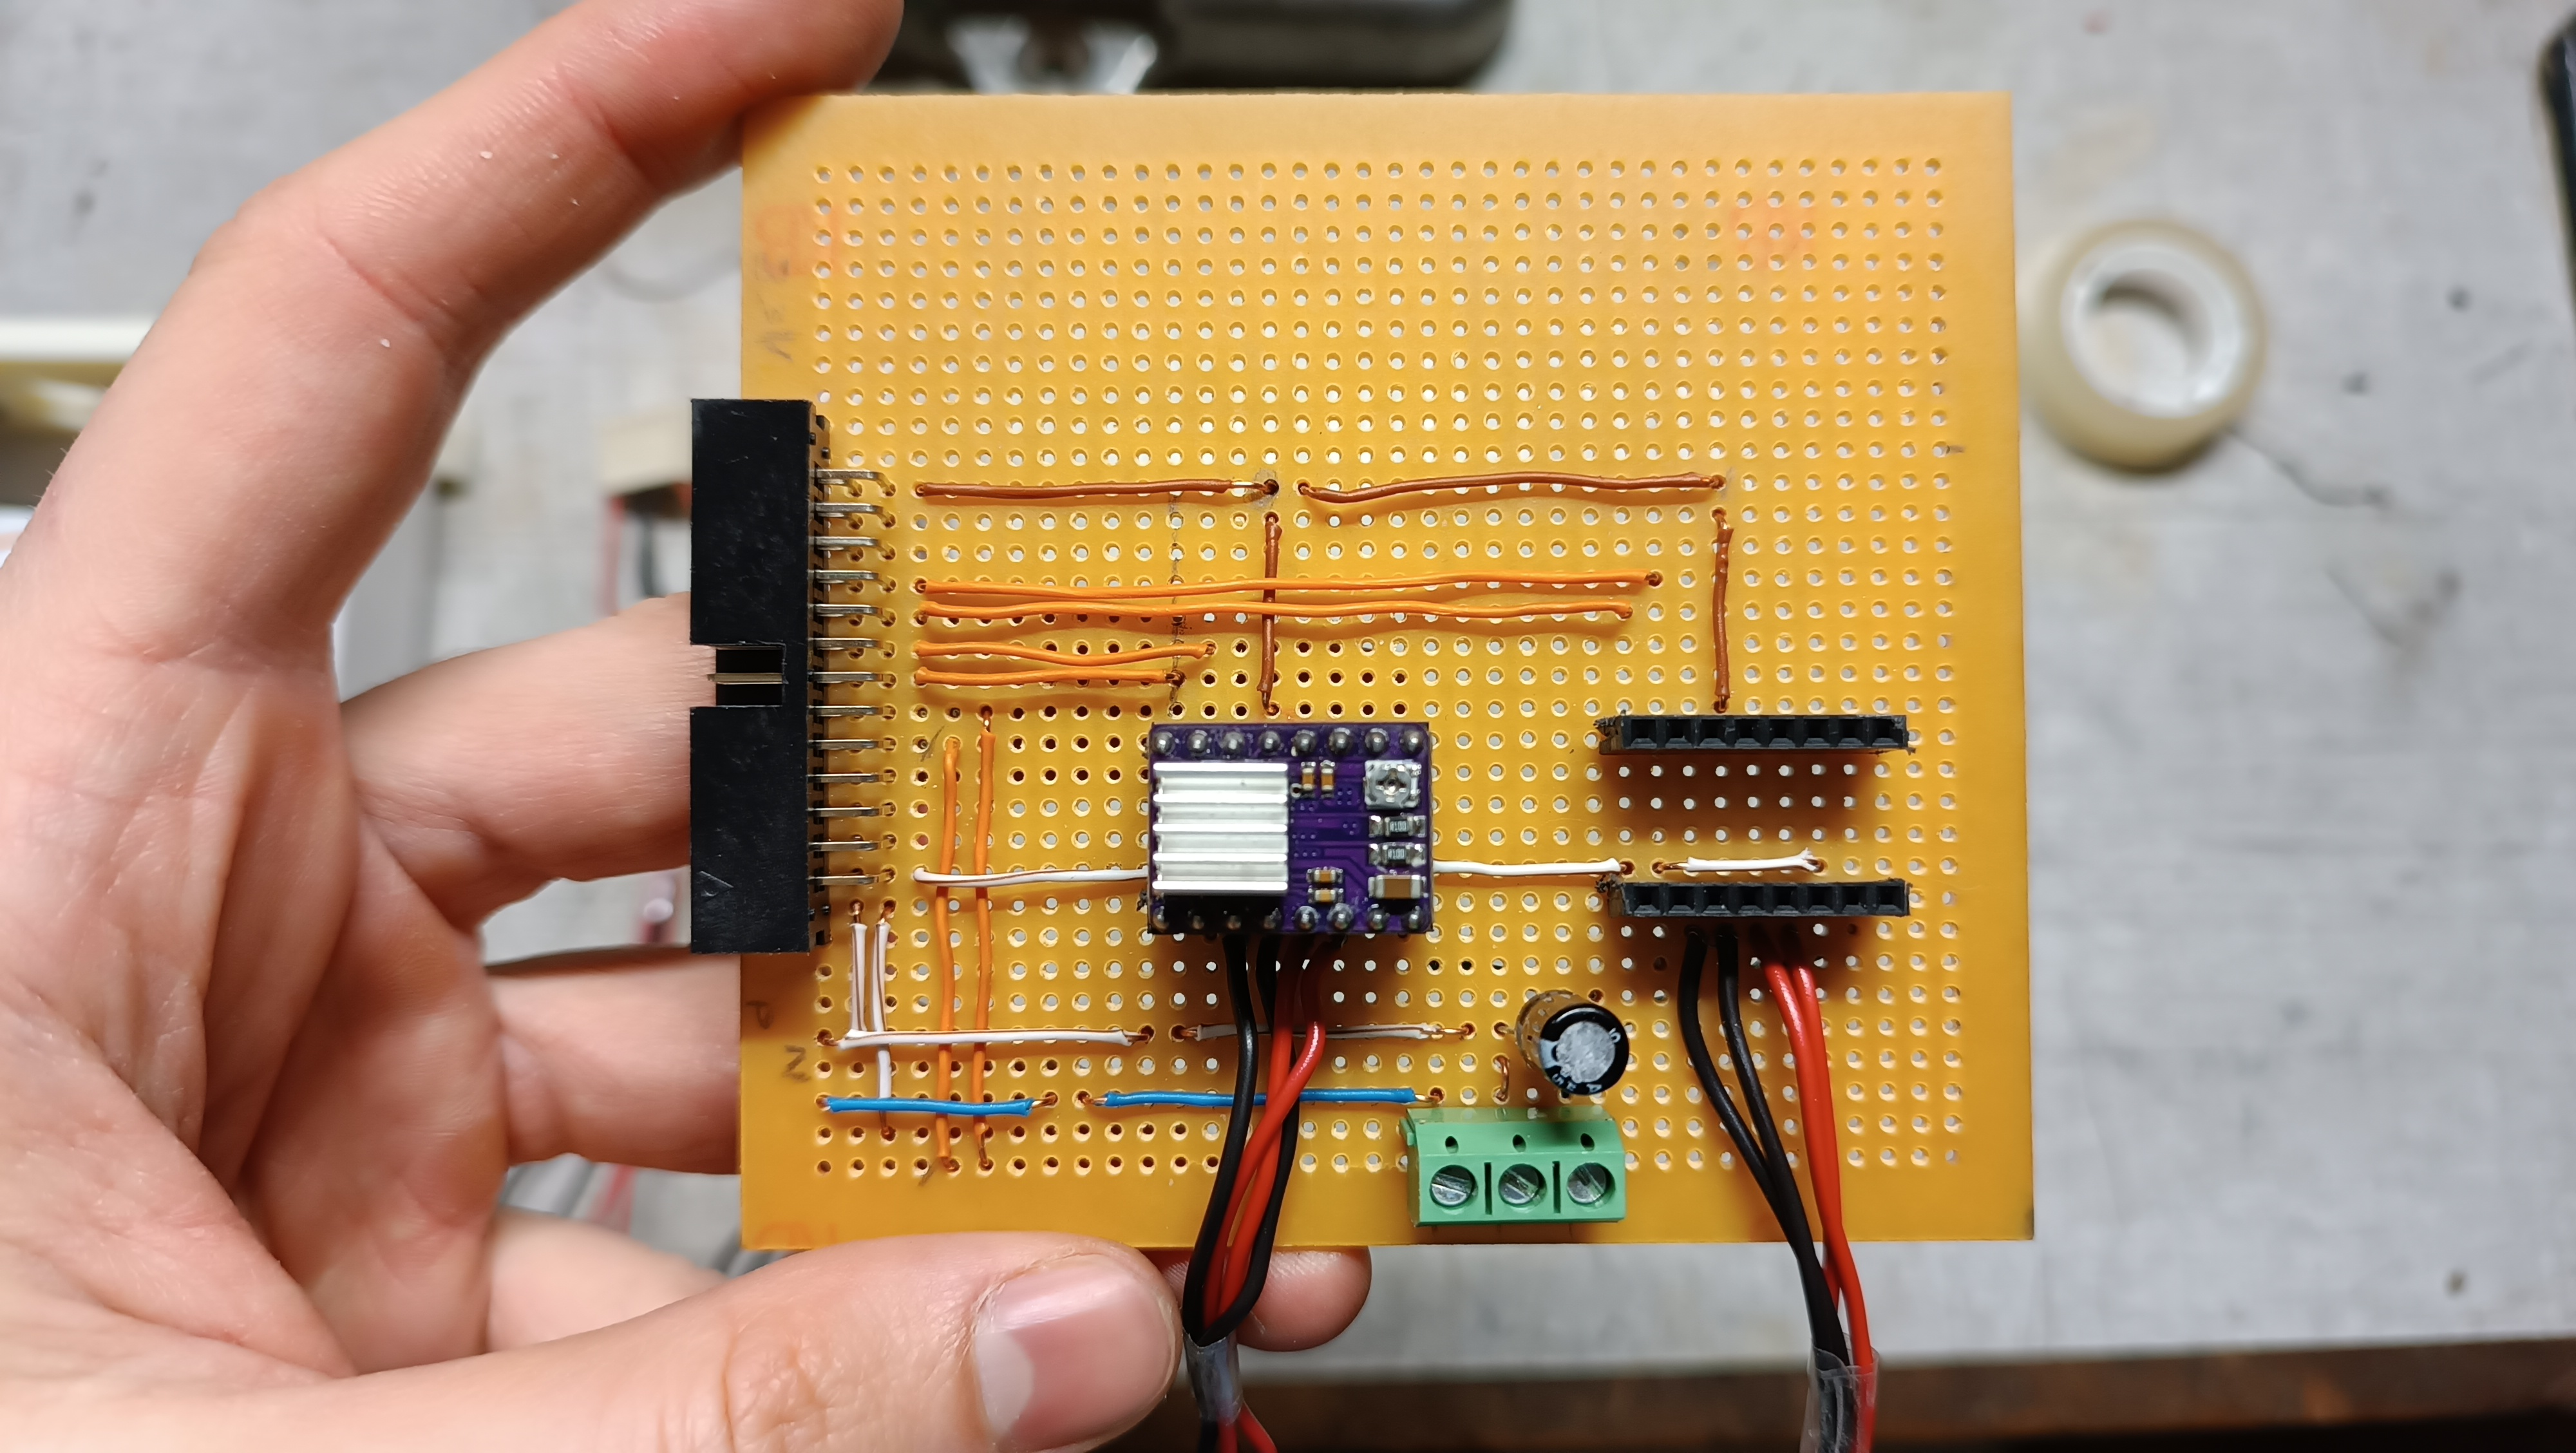
\includegraphics[width=0.9\textwidth]{placa.jpg}
     \caption{\textbf{Horiba PTI QuantaMaster 400 picture}. \todo{maybe pasar a apéndice} (\textbf{A}) Picture of the whole spectrometer. Circled in red the monochromators' motors and limit switches. (\textbf{B}) Stepper motors pin diagram. The only used pins for the refurbished version are 1 and 7, and 3 and 5, which correspond to each motor winding respectively. (\textbf{C}) Limit switches pin diagram.}
     \label{fig:placa}
\end{figure}


\subsection{Software} \label{sec:software}

Para reemplazar el rol que cumplía el \textit{software} FelixGX en el espectrofluorímetro original desarrollamos dos paquetes de Python de control de instrumental y adquisición de datos \cite{napoli_tdinapoli_2024,grecco_hgrecco_2024}.
El código corre en la microCPU de la RP y permite controlar al espectrofluorímetro a través de una interfaz de programación de aplicaciones (API) y una interfaz gráfica simple (GUI) desarrollada con el paquete \textit{IPython's Jupyter Widgets}.
El programa conformado por ambos paquetes está compuesto de cuatro capas principales (\textbf{Fig. \ref{fig:code}}):

\begin{itemize}
     \item \textbf{RedpiPy}: Es uno de los dos paquetes que desarrollamos. Consiste en un \textit{wrapper} de la API original de la RP que resulta en que el código esté mejor organizado para hacer una aplicación en Python. Se compone de funciones y clases que permiten manejar el \textit{hardware} de la RP a bajo nivel, como \textit{RPDO} que controla los pines digitales, así como algunas clases de más alto nivel como \textit{Oscilloscope} que permite manejar el osciloscopio.
     \item \textbf{Clases de dispositivos}: Controlan componentes individuales del espectrofluorímetro, como los monocromadores, el láser pulsado, y los motores de los monocromadores permitiendo la el control de todas las partes por separado. 
     \item \textbf{Clase Spectrometer}: Coordina el \textit{hardware} para protocolos de medición específicos (por ejemplo, adquirir un espectro de emisión). Es fácil de usar desde un script en Python o desde la línea de comandos. Además, es la encargada de contar los pulsos de voltaje negativo registrados por el PMT. Es utilizada por la interfaz gráfica.
     \item \textbf{Interfaz gráfica (GUI)}: proporciona herramientas de adquisición similares a las de FelixGX. Se accede a través de la web y utiliza el paquete IPython's Jupyter Widgets.
\end{itemize}

Gracias a este diseño la parte del código que implementa el control del instrumento es completamente general y está desacoplada del resto, por lo que debería funcionar para cualquier modelo de espectrofluorímetro cuyos monocromadores sean controlados por motores por paso, y la señal de luminiscencia se lea con un PMT.
Por otro lado, la API pública le permite al usuario avanzado crear sus propios protocolos de medición que se pueden ejecutar sin la supervición de un operario.
Tanto \textit{RedpiPy} como \textit{RefurbishedPTI} (el paquete que controla al espectrofluorímetro) se encuentran públicos en repositorios de \href{https://github.com}{GitHub} con sus respectivas instrucciones de instalación. 
El apéndice \ref{apendice:instrucciones_uso} explica detalladamente algunos ejemplos que muestran cómo medir un espectro estacionario y el tiempo de vida para distintas longitudes de onda, ambos a través de la API y de la GUI.


%\todo{ \\
%capacidades del software \\
%\\
%Jerarquía de clases API para desacoplar. Extensión del software: sirve para espectrofluorímetro genérico siempre y cuando tengas motor por pasos y pmt.\\
%\\
%quien cuenta los picos, (mencionar que hay analisis de picos más adelante)\\
%\\
%Modos de uso, API GUI (capacidades, más detallado en apéndice).\\
%}

\begin{figure}[h]
     \centering
     \caption{\todo{cambiar esta figura} \textbf{Structure of the software}. Each element of the software is ordered from high level (\textbf{top}) to low level (\textbf{bottom}). Inside the dashed line black box In yellow, the two ways the end user can interact with the software. In orange, the refurbished instrument API classes. In red, the RP's hardware API.}
     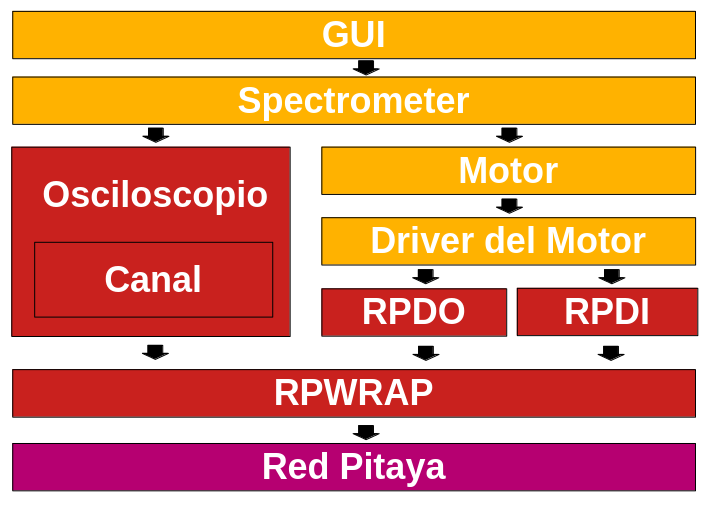
\includegraphics[scale=0.3]{software-diagram.png}
     \label{fig:code}
\end{figure}

%\todo{introduccion a medicion de tiempos de vida}

El tiempo máximo de adquisición de 8 ms ofrece una ventana suficientemente amplia para la mayoría de los materiales luminiscentes. 
Como se mencionó anteriormente, cuando se requiere medir tiempos de vida mucho más largos al tiempo de adquisición máximo (0.5 ms), la ventana de detección puede desplazarse respecto al \textit{trigger} para cubrir un rango más amplio. 
El \textit{software} permite configurar la cantidad de veces que se mide cada ventana de 0.5 ms, lo que hace posible construir una curva de decaimiento más extensa de la luminiscencia.

%\todo{ \\
%explicar que es lo mismo que antes salvo que se usa el trigger.\\
%Explicar funcionamiento de las pantallas y offsets \\
%}

\section{Protocolo de medición estática}

El espectro estático de emisión(excitación) de una muestra consiste en la medición de su intensidad de luminiscencia al iluminar(observar) en una longitud de onda fija, y observar(iluminar) barriendo un rango de longitudes de onda.
Por lo tanto, antes de iniciar una medición deben estar definidos sus parámetros que en este caso son el tiempo de integración $t_{int}$, la longitud de onda de iluminación(medición) $\lambda_e$, y la longitud de onda inicial $\lambda_i$ y final $\lambda_f$ del barrido, así como el paso $\lambda_s$ entre cada medición de intensidad.
En el caso de tomar un espectro de UCNPs, dado que la iluminación proviene del diodo láser de 976 nm, también es necesario configurar la potencia óptica de excitación.

Una vez configurados los parámetros, el espectrofluorímetro debe realizar los siguientes pasos:

\begin{enumerate}
     \item \textbf{Inicializar los monocromadores} haciendo girar los motores en una misma dirección hasta que la señal del fin de carrera de cada uno sea de 5 V. Esto sirve para que la longitud de onda guardada por el \textit{software} coincida con la real.
     \item \textbf{Mover el monocromador estático} de emisión(excitación) hasta $\lambda_e$. 
     \item \textbf{Mover el monocromador dinámico} de excitación(emisión) hasta $\lambda_f$ en pasos de $\lambda_s$. Para cada longitud de onda los pasos (a) y (b) se deben repetir (\textbf{Fig. \ref{fig:diag_medicion_estatica}A}) $n$ veces, donde $n$ es tal que $n \times t_{max} \geq t_{int}$ y $t_{max}$ es el máximo tiempo de medición que soporta la RP (8 ms):
     \begin{enumerate}
          \item Medir la señal del PMT.
          \item Contar los picos en esa señal y acumularlos. Al finalizar, el resultado es la cantidad de picos (fotones) contados por segundo.
     \end{enumerate}
\end{enumerate}

\noindent Una vez que el monocromador dinámico llega a $\lambda_f$ la cantidad de cuentas por segundo para cada longitud de onda se guarda en una tabla y termina la medición.
Al caracterizar UCNPs la excitación se da a través del láser externo, por lo que se deben configurar sus parámetros independientemente y el monocromador de excitación no toma ningún rol.
Como siempre se miden pantallas enteras, los tiempos de integración posibles siempre son múltiplos de 8 ms.
Sin embargo, los tiempos de integración necesarios suelen ser típicamente del orden de los segundos, dos o tres órdenes de magnitud mayores a la duración de la pantalla.
Además, los datos también contienen el tiempo de integración para cada punto con un error de $\sim 15$ ns.
En caso de que sea necesario medir con un tiempo de integración más preciso, esto se puede lograr modificando levemente el \textit{software}.

\begin{SCfigure}
     \centering
     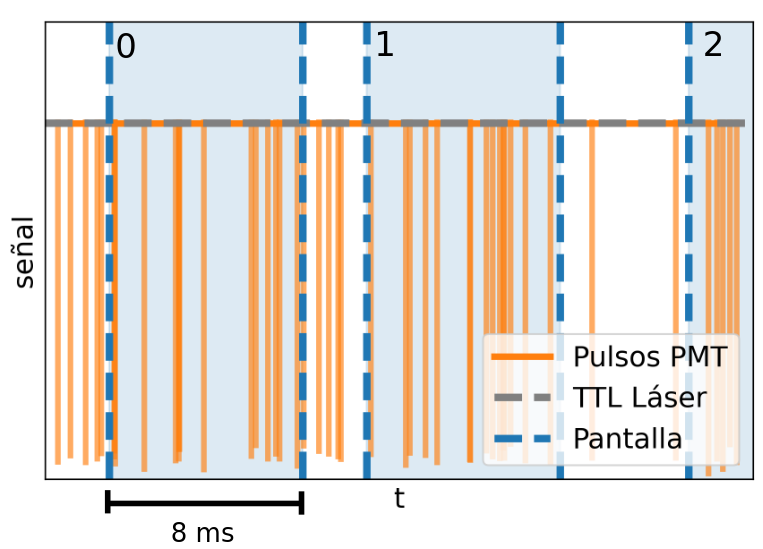
\includegraphics[width=0.6\textwidth]{diag_medicion_estatica.png}
     \caption{\textbf{Diagrama de medición estática}}
     \label{fig:diag_medicion_estatica}
\end{SCfigure}

\section{Protocolo de medición dinámica} \label{sec:proceso_dinamico}

La medición de los tiempos de vida de las nanopartículas de \textit{upconversion} se realiza mediante la técnica de TCSPC (ver sección \ref{sec:intro_tcspc}).
Dado que estos tiempos de vida están en el rango de cientos de microsegundos, no son necesarios varios de los componentes de electrónica rápida típicos de la TCSPC utilizada en mediciones en el rango de nanosegundos, como el CFD y el TAC, los cuales son reemplazados por componentes más simples y menos costosos.
Contradictoriamente, esto hace que no se puedan caracterizar UCNPs utilizando equipos de fluorescencia de uso general, dado que el tiempo total de adquisición necesario difiere en órdenes de magnitud.
En nuestro caso, llevamos a cabo la técnica utilizando el trigger configurable a través de las entradas analógicas de la RP, y la señal TTL proveniente de la fuente de alimentación del láser.
Otra diferencia con TCSPC tradicional es el modo de excitación de la muestra.
Como la mayoría de fluoróforos orgánicos presentan su luminiscencia a través de la excitación de transiciones dipolares eléctricas, pérdia de energía por fonones, y re-emisión a través otra transición dipolar, todos fenómenos que ocurren en el orden de los nanosegundos, es posible estudiar su espectro dinámico al excitar con un pulso del láser.
En el caso de las UCNPs, su luminiscencia se da por la dinámica no lineal de la interacción entre sus dopantes lantánidos (Yb$^{+3}$ y Er$^{+3}$), procesos que incluyen la excitación sucesiva sus electrones y por lo tanto ocurren en el orden de los microsegundos.
Por este motivo, es necesario iluminar a la muestra por algunos milisegundos para asegurarse de llegar al estado estacionario del sistema antes de medir su decaimiento.
Esto se hace aprovechando la función de alimentación pulsada (\textit{Quasi Continuous Wave} ó QCW) que ofrece la fuente ITC4020, la cual permite configurar frecuencia de pulsado $\nu$, y ciclo de trabajo $dc$ (\textbf{Fig. \ref{fig:diag_medicion_dinamica}}).

Para hacer una medición de TCSPC es necesario definir la longitud de onda $\lambda$ en la que se detectará la emisión, el intervalo de tiempo $t_{max}$ en el que se van a contar los fotones luego del trigger, y la cantidad de veces $n$ que se va a medir ese intervalo.
Entonces, el protocolo para realizar la medición es:

\begin{enumerate}
     \item \textbf{Iniciar el láser en modo QCW} para que se prenda y se apague con frecuencia $\nu$ y ciclo de trabajo $dc$.
     \item \textbf{Configurar }
\end{enumerate}


\begin{figure}
     \centering
     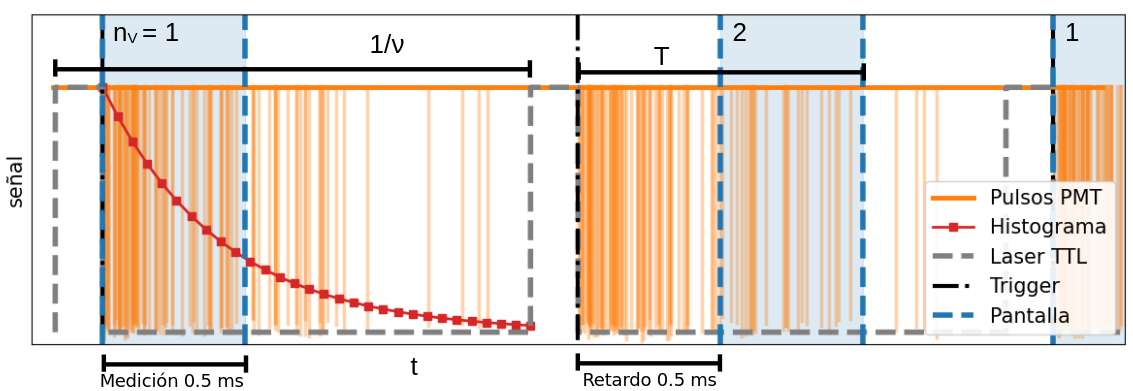
\includegraphics[width=\textwidth]{diag_medicion_dinamica.png}
     \caption{\textbf{Diagrama de medición dinámica}}
     \label{fig:diag_medicion_dinamica}
\end{figure}
